\section{Application Structure}
\label{sec:application_structure}

Web applications have a single point of entry, a hostname, that is translated into an IP address. The IP address points to a server, which then handles HTTP requests. This means that a server solution is needed. Server solutions can either be a singleton or a distributed with multiple servers. Singleton server solutions are based on having one server that handles all incoming requests. This means that singleton server solutions are vulnerable to DoS, through HTTP requests, but provides consistency.

\begin{figure}[htb]
    \centering
    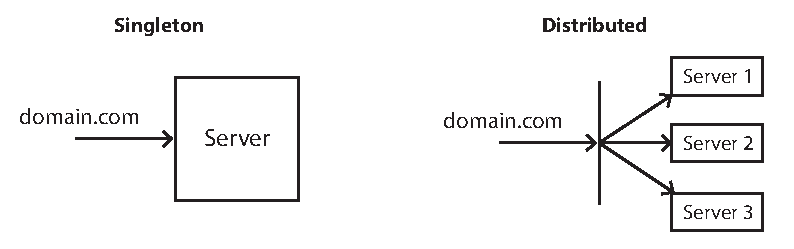
\includegraphics[width=\textwidth]{gfx/server_solutions.pdf}
    \caption{Server Solutions to \projectname{}}
    \label{fig:server_solutions}
\end{figure}

Distributed server solutions contain several servers possibly on several locations, meaning that DoS will be harder to perform, since there is no single point of failure. However, this solution cannot ensure consistency and adds complexity. The two solutions are graphically displayed in Figure~\ref{fig:server_solutions}. A singleton solution has been chosen due to; consistency and simplicity. This singleton solution will be denoted as Master or \deno{M}.

The application is required to handle communication with drones, as defined by Acceptance test[3]. In case of the communication being disabled, this might end up with a drone crash. The technical limitations of antennas for digital wireless communication, sets a constraint for the availability of drones. Assuming there exists no antenna to cover the physical area of our problem domain, it is necessary to have a distributed antenna setup in order to cover the whole physical area of the problem domain. This leads to the structure shown in Figure~\ref{fig:antenna_structure}.

\begin{figure}[htb]
    \centering
    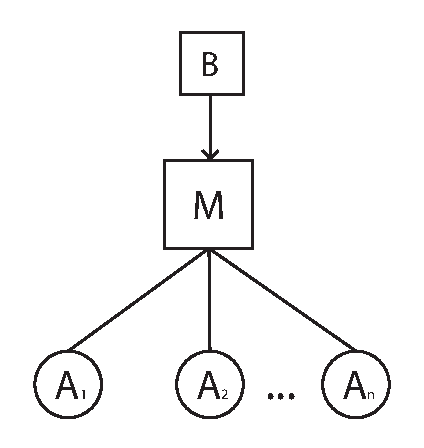
\includegraphics[width=\textwidth]{gfx/antenna_structure.pdf}
    \caption{Antenna Solutions to \projectname{}}
    \label{fig:antenna_solutions}
\end{figure}

If all communication with the drones goes through \deno{M}, this would create a single point of failure. This means that, if \deno{M} crashes at any point, all communication with the drones will be disabled. Providing the antennas with processing power and opportunity to communicate directly with the user would solve this issue, since communication would not go through \deno{M}. If an antenna crashes only the drones connected to that antenna would be disconnected, leaving the drones connected to other antennas untouched. This could be achieved by distributing some of the communication from \deno{M}. This is solved by combining the antennas with distributed processing units, which will be denoted as Slaves or \deno{S}, as shown in Figure~\ref{slave_structure}.

\begin{figure}[htb]
    \centering
    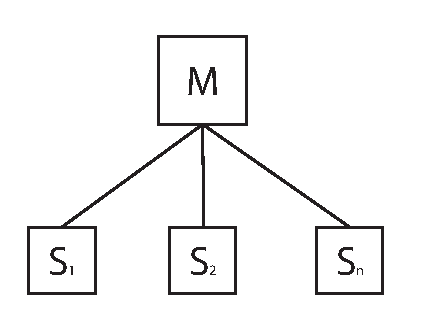
\includegraphics[width=\textwidth]{gfx/slave_structure.pdf}
    \caption{Slave Structure of \projectname{}}
    \label{fig:slave_structure}
\end{figure}
<< Figure slave_structure.pdf >>

% The architecture of \projectname{} differs from other web applications due to the fact that there exists two different type of servers.
% The architecture can be seen in figure~\ref{fig:system_architecture}.
% The server where the web application is running is called Master denoted M.
% For each drone in the system there is a Slave denoted S.
% On both M and S there exists daemons which is responsible for different tasks, however there is some similarity in the tasks they perform.
% These tasks can happen at anytime therefore the program needs to be running at anytime. These daemons are denoted D.
% Each user have a browser they view the application through this is denoted B.
% It is M's responsibility to communicate with every S in the system.
% S is responsible for all communication with the drone it is parred with.

% When a user wants to interact with a drone in the system a session key is needed.
% Such a session key is generated by S and then given to B through M.
% When both B and S have the same session key it is possible for them to communicate without M.
% This ensures that M does not become a bottleneck for controlling and streaming from drones and it reduces latency.
% When a new drone is added it is controlled by its S. This ensures that the system can scaled out and not have to scale up.
% Scale out means using more than one server where scale up means adding more processors, ram etc. to the server so it can handle more by itself.
% M does not handle commands and streaming, and every drone in the system have their own S.
% This makes the application architecture scalable because it removes bottlenecks from both M and S's.

% \begin{figure}[htb]
%     \centering
%     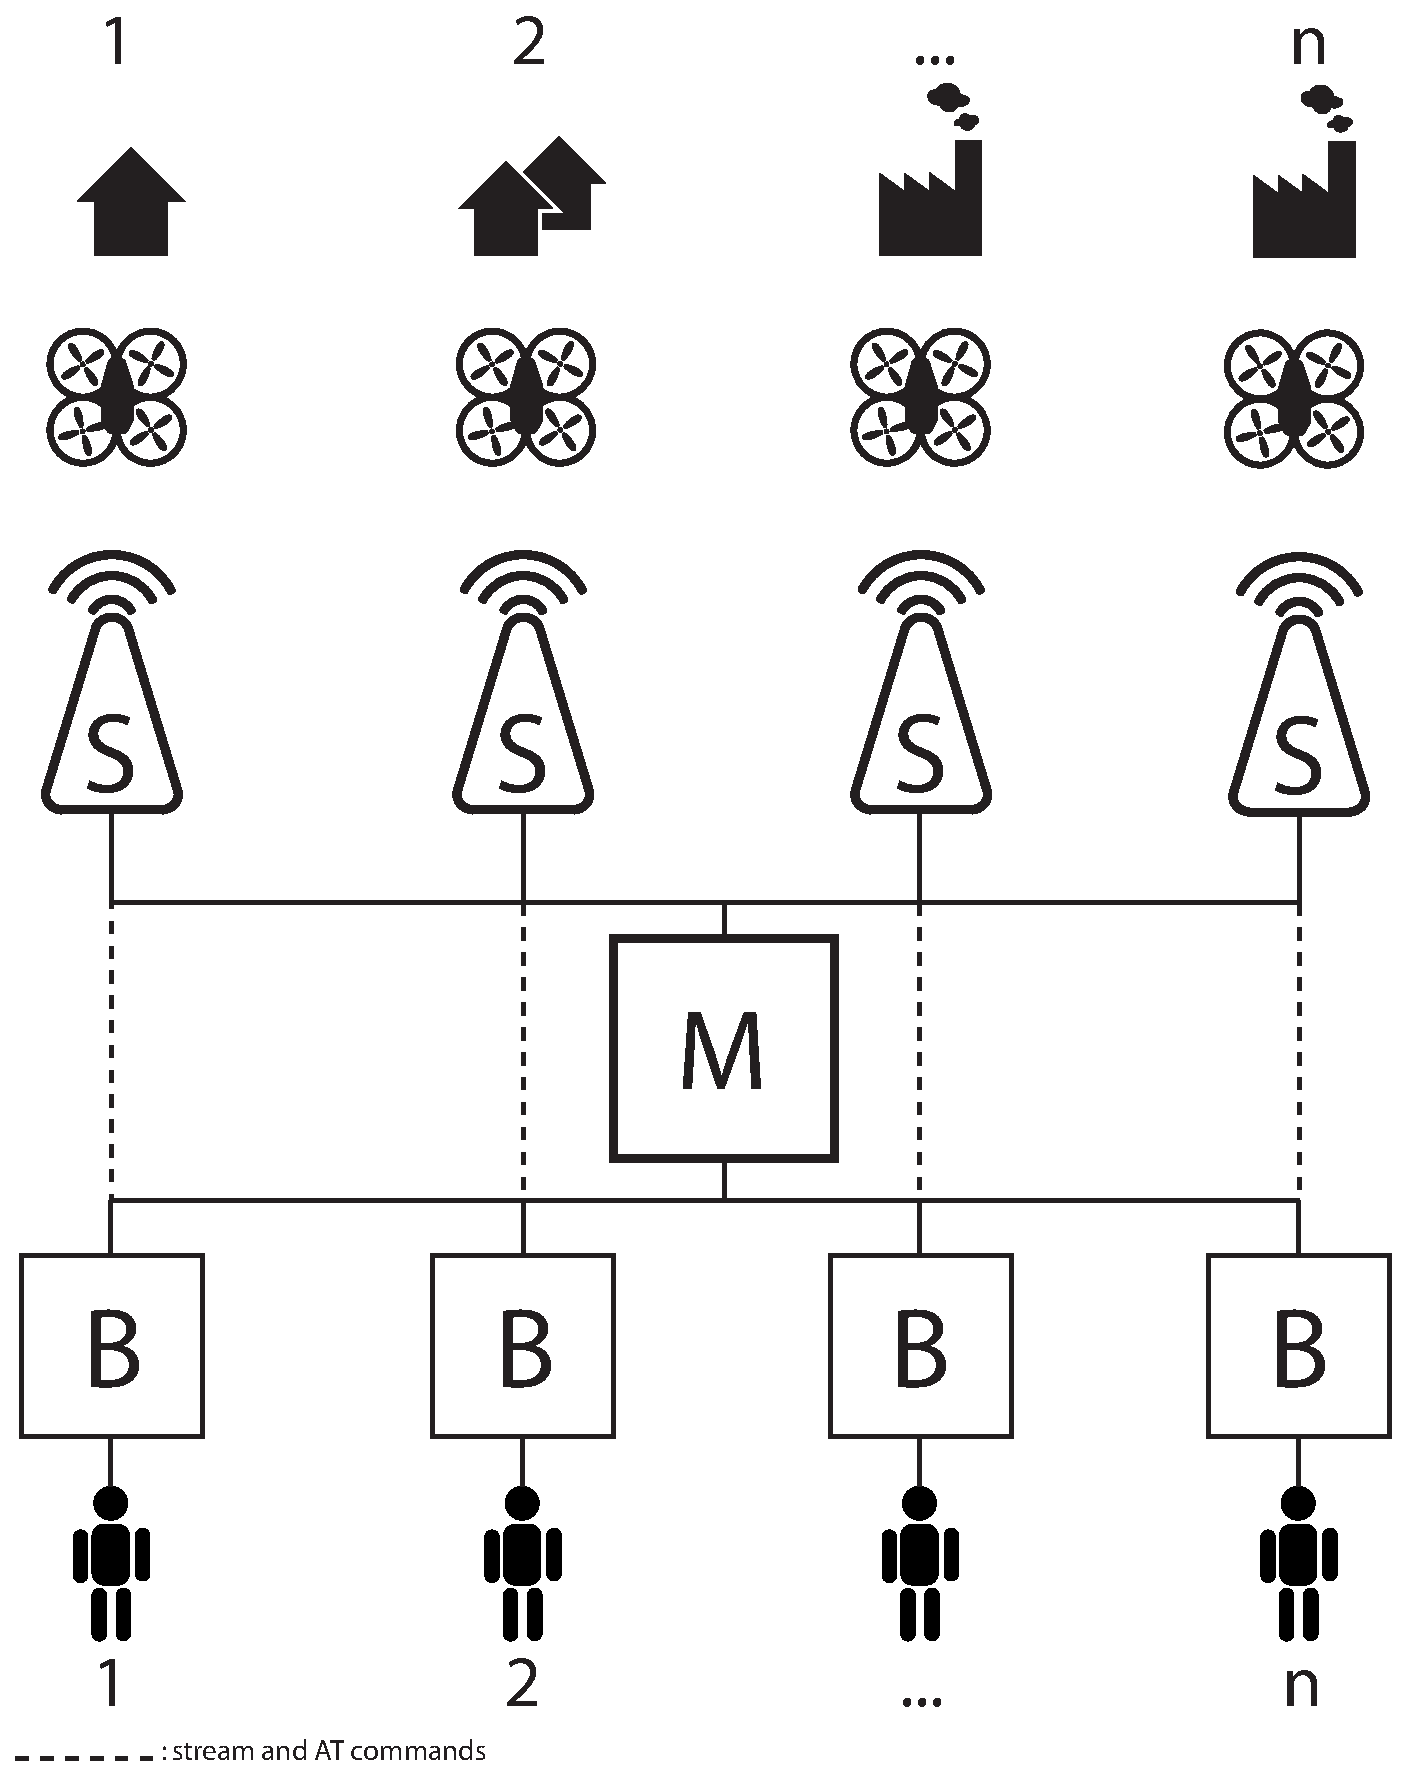
\includegraphics[width=\textwidth]{gfx/system_architecture.pdf}
%     \caption{System architecture of \projectname{}}
%     \label{fig:system_architecture}
% \end{figure}

% The system only uses one M. This can also be seen the bottleneck of the system.
% If M crashes all S's and B's will have to wait for M to come back up.
% One alternative could be running with more M's and in that way scale out.

% There is always one S for each drone connected to the system.
% In this way the system is scaled out.
% This ensures that any S is not likely to become a bottleneck.
% This was done because the drone uses wireless network which is short ranged and the drone is the host which means that the server needs one wireless connection for each drone it have to transmit to.
% One alternative could be only running with one S at each company and just scale it up.
% The problem with this is the server will need a wireless connection for each drone it have to control and it have to be in range.

% Daemon is a background process on a Linux system.
% Daemons are used when it is needed that a process is running at all times.
% In \projectname{} there are both the session key system which both resides on M and S and a policy file system for Adobe Flash on S.
% Both of these processes needs to be running at all times for the user to interact with the drone on S.